\chapter[Dados do Processo GPeQ]{Dados do Processo GPeQ}
\label{chap:dados}
	
	\section[Definição]{Definição}
	\label{sec:dados_definicao}

	Se qualquer departamento de produção deseja entender sua contribuição para a organização de que faz parte, deve responder a duas questões. A primeira é sobre o papel da função produção, isto é, que papel se espera que ela desempenhe dentro da empresa? Segunda, quais os objetivos específicos de desempenho utilizados pela empresa para avaliar a contribuição da produção em suas aspirações estratégicas? Ambos esses assuntos são de importância vital a qualquer operação. Sem a apreciação de seu papel dentro da empresa, as pessoas que dirigem a produção nunca podem estar seguras de que, realmente, estão contribuindo para o sucesso da empresa a longo prazo. Em nível mais prático, é impossível saber se uma operação é bem-sucedida ou não, se os objetivos específicos de desempenho em relação aos quais seu sucesso é mensurado normalmente não estão claramente explicitados. \cite{slack}

	\section[Recursos Transformadores]{Recursos Transformadores}
	\label{sec:dados_transformadores}

		São aqueles que agem sobre os recursos a serem transformados. Eles atuam de forma “\emph{catalisadora}”, ou seja, fazem parte do processo de produção, mas não sofrem transformações diretamente, apenas permitem que a transformação aconteça. Os recursos transformadores, geralmente incluem: 

		\begin{itemize}
			\item{Instalações, ou seja, os prédios, máquinas, equipamentos, terreno etc;}
			\item{Conhecimento, representado pela tecnologia do processo de produção e a necessidade do domínio da técnica \emph{(know-how)};}
			\item{Funcionários para operar, manter, planejar e administrar a produção.}
		\end{itemize}

		- Contexto \textbf{Bob’s}:

		As instalações físicas do \textbf{Bob’s} possuem características que o faz diferenciar-se de suas próprias franquias, ou seja, um quiosque do \textbf{Bob’s} não possui a mesma estrutura que uma loja convencional.
		
		Nas redes do \textbf{Bob’s} a estrutura organizacional não difere de outros restaurantes \emph{fast foods} famosos. Tem-se os gerentes de produção, funcionários de atendimento, funcionários de produção, entre outros. Como entrada, há fornecedores de carne, legumes, fritas que normalmente são distribuídas das matrizes centrais. O transporte de matérias prima é rodoviário, o que requer um planejamento prévio para que não ocorra o atraso nas entregas.


	\section[Recursos Transformados]{Recursos Transformados}
	\label{sec:dados_transformados}

		São aqueles que serão convertidos por meio de um processo de produção. Geralmente são um composto de: 

		\begin{itemize}
			\item{Matérias-primas e Componentes;}
			\item{Informações;}
			\item{Consumidores.}
		\end{itemize}
		
		- Contexto \textbf{Bob’s}:

		São diversas as matérias primas para a produção de um sanduiche no \textbf{Bob’s}. Desde a carne pré frita até a alface fresca. Não apenas para o sanduiche, mas para os diversos outros produtos oferecidos pela empresa. Ou seja, existe toda uma logística por trás até mesmo do transporte desses materiais. Principais matérias-primas utilizadas: Pão, hambúrguer, alface, tomate, queijo (diversos tipos), bacon, ovo, leite e sorvete.

		O público alvo de um \emph{fast food} pode variar até mesmo de região, mas geralmente atende a todos (crianças, adolescentes, jovens, adultos e idosos). É normal existirem produtos especializados para determinado público, como os pratos personalizados de forma a trazer alegria a uma criança. Mas, normalmente a maioria dos produtos estão padronizados para atender as exigências das demais faixa etárias.

		De modo geral, recursos transformados e transformadores tendem a compor a estrutura de produção e consumo de um bem ou serviço. Para este contexto, o \textbf{Bob’s}, como uma empresa de \emph{fast food}, tem como objetivo a produção rápida e eficiente de seus produtos. Isso significa que boa parte de suas matérias primas possuem características de negócio que se adequam ao contexto da empresa. Por exemplo, carnes e batatas são pré fritas para que levem menos tempo para estarem prontas durante o processo de produção, sorvete são mais cremosos para produção dos \emph{milk shakes} para não sofrer modificações na consistência do produto final entre diversas outras características.

	\section[Estratégia da Produção]{Estratégia da Produção}
	\label{sec:dados_estrategia}

		A estratégia de produção é definida como um padrão de decisões e ações estratégicas que define o papel, os objetivos e as atividades da produção. Normalmente, estratégias significam que as decisões tem um efeito abrangente na organização ao qual a estratégia se refere, definem a posição da organização relativamente a seu ambiente e aproximam a organização de seus objetivos de longo prazo. No entanto, não existe um padrão universal de como essas definições estratégicas devem ser realizadas. Mas sim perspectivas que são ilustradas a seguir:

		\begin{figure}[h]
			\centering
			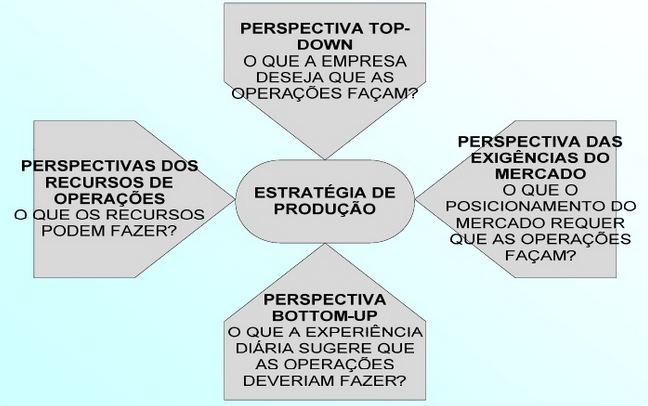
\includegraphics[scale=0.6]{dados1}
			\caption[Estratégia de Produção]{Estratégia de Produção. \cite{slack}}
			\label{fig:dados1}
		\end{figure}

		\subsection[Perspectiva Top-Down]{Perspectiva \emph{Top-Down}}
		\label{sec:dados_perspNorte}

			A perspectiva top-down define a característica de que a empresa deseja que as operações façam. Para o contexto do \textbf{Bob’s} tem-se:

			Como estratégia corporativa do grupo de serviços, a especialização em fornecimento em comida rápida. Em que é caracterizado pelo atendimento e produto final rápido e de qualidade.

			Como estratégia de negócio para o consumidor estão envolvidos o rápido crescimento no volume de produção, a variedade de opções ofertadas e o serviço rápido e de qualidade.

			Como estratégias de operação, a velocidade de produção das diversas etapas de produção, intolerância a fator de baixa qualidade do produto final e estabelecimento de um atendimento fluido.

		\subsection[Perspectiva Bottom-Up]{Perspectiva \emph{Bottom-Up}}
		\label{sec:dados_perspSul}

			A perspectiva bottom-up define a característica que a experiência diária sugere para as operações. Para o contexto do \textbf{Bob’s} tem-se:

			Por possuírem produtos de fácil (e rápida) produção, isso permite-lhes um produto final de excepcional rapidez para os consumidores. 

			No entanto, os preços são fixos de acordo com padrões da matriz central, o que significa que franquias não devem sobrepor este padrão.

			Isso leva a empresa a se adequar à realidade de seus recursos disponíveis, desde que não afete a qualidade da marca de forma geral.

			\begin{figure}[h]
				\centering
				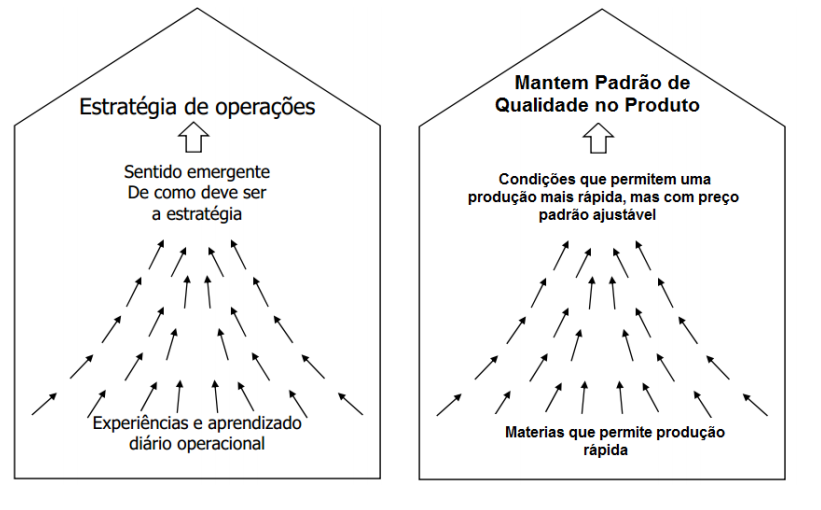
\includegraphics[scale=0.6]{dados2}
				\caption[Esquema representativo da Perspectiva Bottom-Up]{Esquema representativo da Perspectiva Bottom-Up. \cite{slack}}
				\label{fig:dados2}
			\end{figure}

		\subsection[Perspectiva das Exigências do Mercado]{Perspectiva das Exigências do Mercado}
		\label{sec:dados_perspLeste}
			
			A perspectiva de requisitos de mercado define a característica de que a empresa é satisfeita no mercado a que está servindo seus produtos e/ou serviços. Para o contexto do \textbf{Bob’s} tem-se:

			Existem requisitos que são existências dos clientes de um \emph{fast food}, são eles: Preço mediano, alta qualidade, entrega muito rápida, produto (consumível) confiável, produto e serviço pouco inovador, ampla variedade de escolha de produto e possibilidade de flexibilidade (Quantidade).

			Portanto, critérios que a \textbf{Bob’s} trabalha para atender relacionam-se a:

			\begin{itemize}
				\item{Custo dos produtos;}
				\item{Qualidade dos produtos e serviços;}
				\item{Velocidade na produção do produto;}
				\item{Confiabilidade na matéria prima e consequentemente no produto final;}
				\item{Flexibilidade de produto, mas de forma não constante (lançamento de novos sanduiches por exemplo);}
				\item{Flexibilidade de produção;}
				\item{Flexibilidade de volume.}
			\end{itemize}


		\subsection[Perspectiva dos Recursos de Operação]{Perspectiva dos Recursos de Operação}
		\label{sec:dados_perspOeste}

			A perspectiva de recursos da produção define a característica da forma com que a empresa herda, adquire ou desenvolve seus recursos de produção, tendo em vista, a longo prazo, os impactos no sucesso da estratégia. Para o contexto do \textbf{Bob’s} tem-se:

			A \textbf{Bob’s} tenta compreender e desenvolver seus recursos de produção, embora que muitas vezes negligenciados por algumas franquias – por isso da exigência de fiscalização delas, para o bom caráter da marca – é uma perspectiva particularmente importante a ser melhorada para elevar a estratégia da produção dessas franquias. \cite{lamonica}